\documentclass[a4paper,12pt,twoside]{report}

\usepackage{acronym}
\usepackage{url}
\usepackage{cite}
\usepackage{listings}
\usepackage[pdftex]{graphicx}
\usepackage[hang,small,bf]{caption}
\usepackage{styles/tum}
\usepackage{setspace}
\usepackage[german,english]{babel}
\usepackage{float}
\usepackage{floatflt}
\usepackage{fancyhdr}
\usepackage{color}
\usepackage{booktabs}
\usepackage[pdftex,bookmarks=true,plainpages=false,pdfpagelabels=true]{hyperref}	%TODO make yourself familiar with \label, \ref and \hyperref for referencing figures, tables, chapters, etc.
\usepackage{mdwlist}
\usepackage{enumerate}
\usepackage{array}
\usepackage{longtable}
\usepackage[utf8]{inputenc}
\usepackage[capitalize, noabbrev]{cleveref}
\usepackage{wasysym}

% Path for graphics
\graphicspath{{figures/}}

\begin{document}
\setlength{\evensidemargin}{22pt}
\setlength{\oddsidemargin}{22pt}

\def\doctype{Bachelor's Thesis}
\def\faculty{Informatik}
\def\title{Perceptual Losses for Deep Learning on Fluid Simulations}		%TODO add title in English
\def\titleGer{Perceptual Losses für Deep Learning von Flüssigkeitssimulationen}	%TODO add title in German
\def\supervisor{Prof. Dr. Nils Thürey}
\def\advisor{M.Sc. Georg Kohl}
\def\author{Hanfeng Wu}			%TODO add author name
\def\date{15.09.2021}		%TODO add submission / handover date


\hypersetup{pdfborder={0 0 0},
                        pdfauthor={<author>},
                        pdftitle={thesis-ba-wenjie},
                        }

\lstset{showspaces=false, numbers=left, frame=single, basicstyle=\small}

\pagenumbering{alph}

\thispagestyle{empty}

\vspace{4cm}
\begin{center}
\begin{figure}[h!]
    \centering
    
\includegraphics[width=4cm]{TUM_Logo_blau_rgb_p}
\end{figure}
\vspace{5mm}     
\huge FAKULT{\"A}T F{\"U}R INFORMATIK\\ 
\vspace{0.5cm}
\large DER TECHNISCHEN UNIVERSIT{\"A}T M{\"U}NCHEN\\
\vspace{1mm}
\end{center}

\vspace{2mm}

\begin{center}
{\Large \doctype\ in \faculty}
\vspace{10mm}

\begin{spacing}{1.5}
{\huge\bf \title}\\%[3ex]
\end{spacing}

\vspace{10mm}
{\LARGE \author}

\vspace{10mm}

\begin{figure}[h!]
\centering
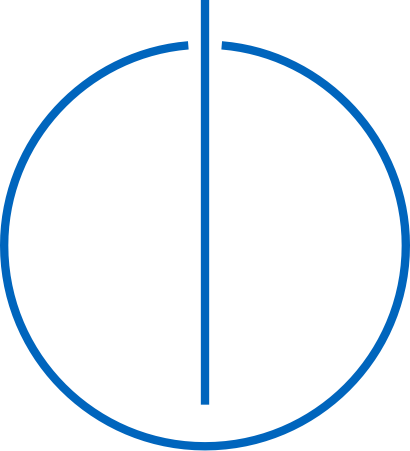
\includegraphics[width=2cm]{FAK_IN_RGB_p}
\end{figure}

\end{center}

\thispagestyle{empty}

\vspace{8mm}
\begin{center}
\oTUM{4cm}

\vspace{5mm}     
\huge FAKULT{\"A}T F{\"U}R INFORMATIK\\ 
\vspace{0.5cm}
\large DER TECHNISCHEN UNIVERSIT{\"A}T M{\"U}NCHEN\\
\end{center}

\vspace{5mm}

\begin{center}
{\Large \doctype\ in \faculty}
\vspace{8mm}

\begin{spacing}{1.3}
{\LARGE \title}\\
\vspace{8mm}

{\LARGE \titleGer}\\
\vspace{8mm}
\end{spacing}

\begin{tabular}{ll}
\Large Author:     & \Large \author     \\[2mm]
\Large Supervisor: & \Large \supervisor \\[2mm]				
\Large Advisor:	   & \Large \advisor    \\[2mm]
\Large Date:       & \Large \date
\end{tabular}

\vspace{1mm}

\begin{figure}[hb!]
\centering
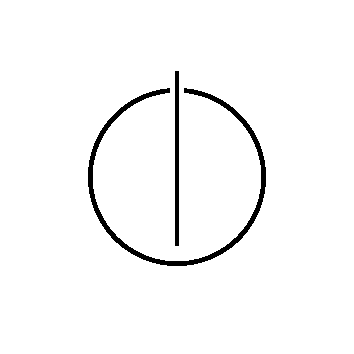
\includegraphics[width=3cm]{InformaticsLogo}
\end{figure}

\end{center}
\newpage
\thispagestyle{empty}
\mbox{}
\clearpage
\thispagestyle{empty}
\vspace*{0.8\textheight}
\noindent
I confirm that this bachelor's thesis is my own work and I have documented all sources and material used.

\vspace{15mm}
\noindent
Munich, \date \hspace{\stretch{1}} \author
\newpage

		%TODO choose one of 'diploma | bachelor's | master's thesis' in the disclaimer file

\newpage
\thispagestyle{empty}
\mbox{}

\chapter*{Acknowledgements}


\pagenumbering{roman}

\selectlanguage{english}
\begin{abstract}

%abstract english

This thesis studies the integration of perceptual loss into several models that are related to fluid simulation. Perceptual losses are used to compare high level differences, while traditional loss functions like MSE and MAE only compare the pixel level differences which is more brute force. 

Now some famous perceptual loss functions like comparing the intermediate layers of pretrained vgg network already improve its performance in some image related tasks.\cite{johnson2016perceptual} We want to show that in the context of fluid simulation, the integration of some pretrained perceptual losses should also outperform the traditional loss functions.

We tested some fluid simulation tasks in SOL\cite{um2020sol} to improve the performance of the percetual loss functions. Meanwhile we also integrate such loss functions into models like autoencoder and superresolution to compare their results with those from the same models but trained by MSE loss functions

Finally we combined the result of SOL and superresolution model to conduct some fluid simulations at a lower cost to show the advantage of integrating perceptual losses in such tasks.

\end{abstract}

\clearpage

\selectlanguage{german}
\begin{abstract}

Diese Dissertation untersucht die Integration von Wahrnehmungsverlusten in verschiedene Modelle, die sich auf die Fluidsimulation beziehen. Wahrnehmungsverluste werden verwendet, um Unterschiede auf hohem Niveau zu vergleichen, während herkömmliche Verlustfunktionen wie MSE und MAE nur die Pixelniveauunterschiede vergleichen, was roher ist.

Einige berühmte Wahrnehmungsverlustfunktionen wie der Vergleich der Zwischenschichten eines vortrainierten VGG-Netzwerks verbessern bereits seine Leistung bei einigen bildbezogenen Aufgaben.\cite{johnson2016perceptual} Wir wollen zeigen, dass die Integration einiger vortrainierter Wahrnehmungsverluste im Kontext der Fluidsimulation übertreffen auch die traditionellen Verlustfunktionen.

Wir haben einige Fluidsimulationsaufgaben in SOL\cite{um2020sol} getestet, um die Leistung der Percetual Loss Functions zu verbessern. Inzwischen integrieren wir solche Verlustfunktionen auch in Modelle wie Autoencoder und Superresolution, um deren Ergebnisse mit denen aus den gleichen Modellen zu vergleichen, die jedoch mit MSE-Verlustfunktionen trainiert wurden

Schließlich haben wir die Ergebnisse von SOL und Superauflösungsmodell kombiniert, um einige Fluidsimulationen zu geringeren Kosten durchzuführen, um den Vorteil der Integration von Wahrnehmungsverlusten in solchen Aufgaben zu zeigen.
%abstract german
\textit{Note: Insert the German translation of the English abstract here.}

\end{abstract}

\clearpage

\selectlanguage{english}


\tableofcontents
\clearpage

\clearpage

\begin{acronym}
\acro{SOL}{Solver in the Loop}
\acro{LSIM}{Learning Similarity Metrics for Numerical Simulations}

\end{acronym}

\pagenumbering{arabic}

\fancyhead{}
\pagestyle{fancy}
\fancyhead[LE]{\slshape \leftmark}
\fancyhead[RO]{\slshape \rightmark}
\headheight=15pt




%------- chapter 1 -------

\chapter{Introductions}

\textit{Note: Introduce the topic of your thesis, e.g. with a little historical overview.}

\section{Perceptual loss functions}

\textit{Note: Describe the problem that you like to address in your thesis to show the importance of your work. Focus on the negative symptoms of the currently available solution.}

\section{Physical simulation}

\textit{Note: Motivate scientifically why solving this problem is necessary. What kind of benefits do we have by solving the problem?}

\section{Deep learning tasks}

\textit{Note: Describe the research goals and/or research questions and how you address them by summarizing what you want to achieve in your thesis, e.g. developing a system and then evaluating it.}

\section{Related Work}

\textit{Note: Describe the outline of your thesis}




%------- chapter 2 -------

\chapter{Perceptual Losses}

\textit{Note: Describe each proven technology / concept shortly that is important to understand your thesis. Point out why it is interesting for your thesis. Make sure to incorporate references to important literature here.}

\section{Learning Similarity Metrics for Numerical Simulations}

\textit{Note: This section would summarize the concept User Feedback using definitions, historical overviews and pointing out the most important aspects of User Feedback.}

\section{VGG-16 loss network}

\textit{Note: This section would summarize the architectural style Representational State Transfer (REST) using definitions, historical overviews and pointing out the most important aspects of the architecture.}

\section{triditional loss function}

\textit{Note: This section would summarize the agile method Scrum using definitions, historical overviews and pointing out the most important aspects of Scrum.}



%------- chapter 3 -------

\chapter{Datasets}

\section{Autoencoder}

\section{Superresolution}

\section{Solver in the Loop}





%------- chapter 4 -------

\chapter{Tasks and Experiments Setup}

\section{Autoencoder}

\section{Superresolution}

\section{Solver in the Loop}



%------- chapter 5 -------

\chapter{Results and Analysis}

\section{Comparison}

\subsection{Numerical evaluation}

\subsection{Time cost evaluation}

\section{Limitaions}





%------- chapter 6 -------

\chapter{Conclusion}
\section{Future work}
\section{Summary}






\appendix

\chapter{e.g. Questionnaire}

\textit{Note: If you have large models, additional evaluation data like questionnaires or non summarized results, put them into the appendix.}


\clearpage

\listoffigures
\clearpage

\listoftables
\clearpage

\bibliography{thesis}
\bibliographystyle{alpha}

\end{document}
